
\chapter{Results}


\section{Kriging and Kalman update validation}

First, the basic approach behind both the kriging interpolation method, and the GEBCO measurement update are validated. To test this, instead of using ICESat-2 data as an input to the kriging step, random point samples of the validation data are taken throughout a single area of interest. This provides a source of exact point data with an RMSE of 0m. Two types of random sampling are considered, randomly across the surface of the validation data, and also samples that are taking along the corresponding ICESat-2 tracks. This simulates the presence of a theoretical perfect ICEsat-2 bathymetry data, and can be compared to the random sampling case to investigate the effect of the tracklines. Any available ICEsat-2 bathymetric data will occur along colinear track lines, and therefore there would always be some spatial gaps in the data even if perfect ICESat-2 data were present along every single tract. By comparing the randomly sampled points to colinear points along the ICESat tracks, we can get an estimation of how much the accuracy is degraded by the data being available only along certain lines. 

A small section of the St. Croix test site is used to implement this trial. First, the raster of the validation data is sampled randomly until there are $10,000$ data points. A larger number of point samples than needed is taken, then of these points $2000$ points are subsampled using the Poisson disk sampling method. 

Figure \ref{fig:truthras-sampling} shows both sets of points that were used as input to the kriging process for the two cases under evaluation. Note that in the bottom figure  there are significant spatial gaps in coverage. This is due to the pattern of ICESat-2 data collection. Even in this theoretical scenario with exact bathymetry values available across the entire track, the spatial anisotropy of the availability of the points can potentially limit the accuracy of the interpolation.

\begin{figure}[h]
    \centering
    \includegraphics{figures/truthraster_sampling_combined.pdf}
    \caption{Top: Random sampling across the area of interest \newline   Bottom: Random sampling only along the ICESat-2 tracks for the site}
    \label{fig:truthras-sampling}
\end{figure}

Because we know the bathymetry points used for this section are exactly the same as the validation data at each point, the \emph{nugget} of the variogram for the Kriging interpolation is set to $0$, so areas that are close known points are given a variance of $0$ by the kriging process. 
\pdfcomment{rerun notebook one more time3}
\begin{table}
\caption{Error between the various data products}
\label{tab:rmse-truth-raster-sampled}
\begin{tabular}{lrr}
 & RMSE & MAE \\
Truth vs 50m bilinear resampling of GEBCO & 6.200386 & 4.697360 \\
Truth vs Kriged raster output & 2.435478 & 1.275817 \\
Truth vs GEBCO+Kriged raster & 1.682143 & 1.057158 \\
\end{tabular}
\end{table}


Table \ref{tab:random-vs-colinear-sampling} shows the results of the two sampling strategies. It can be seen that the more homogenous distribution of bathymetric points in the randomly-sampled data produces a better kriging estimate (RMSE of 3.13m and 4.49m respectively). 

Also of note is that for both cases, the Bayesian combination of the kriging surface with GEBCO produces a better estimate than either on their own. This indicates that there is value in starting from GEBCO and using a bayesian combination approach when compared to either a kriging interpolation of point data or using GEBCO as a data source.


\section{Petten Test Site}
Most research results show that spaceborne lidar is not effective at retrieving bathymetry from very turbid waters. To test the upper limits of this, ICESat-2 data for the coast of Petten, NL was downloaded. As expected, there was no bathymetric signal was found in the ICESat-2 data, likely due to the inability of the laser to penetrate the turbid water. 

However the site provides a useful case to validate the approach of the combination of universal kriging of point bathymetry and Bayesian combination of bathymetry grids. The Dutch government provides a dataset called Jarkus which consists of annual manually surveyed elevations of the coastal zone. These point measurements provide an interesting case to apply the same method but using the Jarkus point measurements as an input instead of ICESat-2 point measurements.

The location of Petten, The Netherlands, located on the Noord-Holland coast, was chosen based on the availability of high-resolution ground-truth bathymetry provided by Van Oord. The survey was performed in 2021, and therefore the 2021 Jarkus points were selected from the dataset. All Jarkus points that overlap the validation data raster were selected. Like the ICESat-2 data points, the Jarkus points are available only along colinear lines. This is due to the measurement method that is based on surveying the dune and seabed starting from a series of fixed measurement poles and then surveying points normal to the shore starting at the reference pole. 


\begin{figure}[h]
    % \centering   
    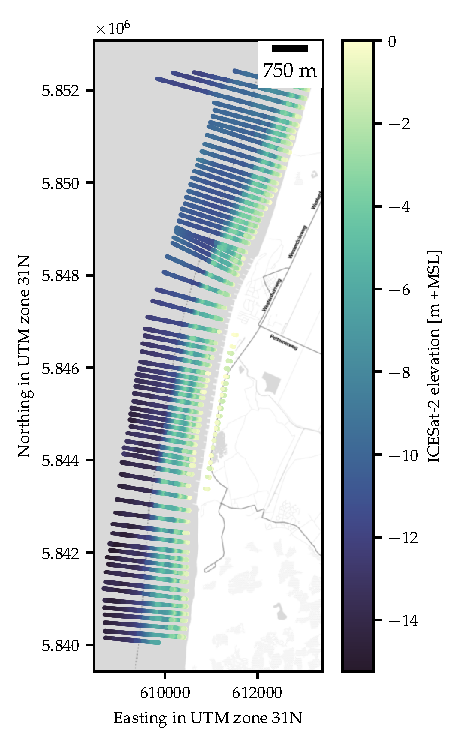
\includegraphics[]{figures/Petten_photon_map.pdf}
    \caption{Jarkus 2021 measurement points within the site}\pdfcomment{figure out how to rotate}
    \label{fig:jarkus-points}
\end{figure}

The Jarkus point measurements were checked for the same error metrics as the ICESat-2 points. The bias plot is shown in Figure \ref{fig:petten-bias-plot}. It is notable that the deviation between the Jarkus data and the survey data is greatest in the in the shallowest part of the nearshore zone; this is likely due to some morphological changes due to wave-drived sediment exchange between the nearshore and the offshore. Both datasets are from 2021, but this area is highly morphologically active. Also, in the deeper part of the study area, the error  between the two datasets decreases significantly. This is likely due to the depth of closure for most profiles in the study area being located between -5 and -10m. 

\begin{figure}[h]
    \centering
    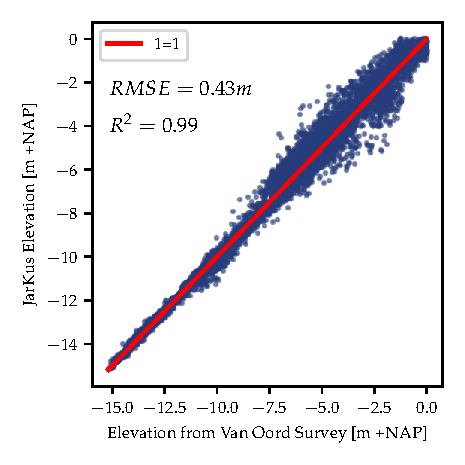
\includegraphics{figures/petten_lidar_estimated_vs_truth.pdf}
    \caption{Petten Test site: Agreement between Jarkus and Van Oord multibeam survey data}
    \label{fig:petten-bias-plot}
\end{figure}

The universal kriging and Kalman Updating concepts are tested for this site. The Jarkus points are used as input to the kriging process instead of ICESat-2 points. It is notable that in this site, the error between GEBCO and the high resolution bathymetry is significantly lower than other test sites. This could be due to higher quality or more recent input data into the GEBCO grid as compared to the other sites. Even with a higher accuracy in the GEBCO data, the kriged bathymetry surface was found to have a lower RMSE and MAE error than GEBCO. However, it was found that the bayesian combination of both of these datasets has the highest accuracy --- indicating that the Bayesian combination of these two datasets provides increases the value compared to either data set individually. 

\begin{table}[!ht]
\centering
\caption{Improvement in error metrics after applying Kalman Updating of kriged data}
\label{tab:Petten_gebco_raster_error}
\begin{tabular}{lrrr}
\toprule
 & RMSE [m] & MAE [m] & ME [m] \\
\midrule
GEBCO & 1.48 & 1.31 & -1.01 \\
Kriging Surface & 1.22 & 0.70 & -0.31 \\
Kalman Output& 1.00 & 0.76 & -0.50 \\
\bottomrule
\end{tabular}
\end{table}



\section{Florida Keys test site}

The area surrounding Marathon Key in the Florida Keys archipelago in Florida, USA was used as one site to test the entire process, including the ICESat-2 signal finding in additional to the kriging and Kalman updating. The area has a wide and relatively shallow ($\mathcal{O}(-10 m +MSL)$) shelf, a microtidal tidal environment, and very clear water, so it is an ideal site for remote sensing of bathymetry. The clear and shallow water provides a relatively strong subsurface signal within ICESat-2 transects. The site was found to have many transects of ICESat-2 data with distinct bathymetric signal. The KDE signal finding approach was applied to all transects within the study area and resulting distribution of the identified signal points is shown in figure \ref{fig:keys-photons}.

\begin{figure}[h]
    \centering
    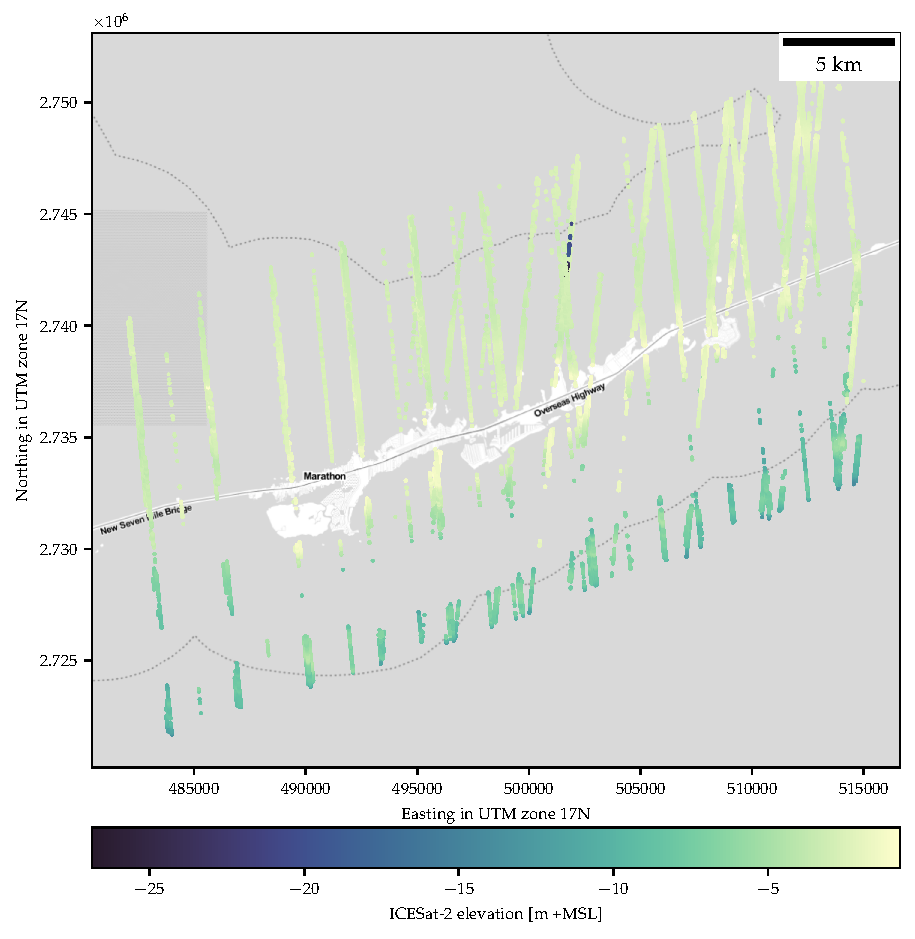
\includegraphics{figures/florida_keys_photon_map.pdf}
    \caption{Marathon Key Site: Location and depth of bathymetric signal points found using KDE signal finding method}
    \label{fig:keys-photons}
\end{figure}

\begin{figure}[h]
    \centering
    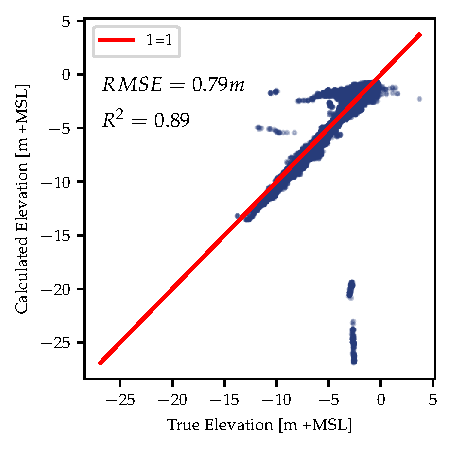
\includegraphics{figures/florida_keys_lidar_estimated_vs_truth.pdf}
    \caption{Marathon Key site: Bias plot showing the results of the KDE signal finding algorithm}
    \label{fig:keys-biasplot}
\end{figure}

Figure \ref{fig:keys-biasplot} shows how the error is distributed within the Florida Keys test site. This site has many transects containing data, but some errors in the signal finding can be seen in this bias plot. There is one cluster of points with a real elevation of -2.5m, while the KDE finding output identifies the seafloor elevation as between -20 and -27m.  The figure also shows a few clusters of points where the seabed location was overestimated slightly. 

However, the kriging process can account for an expected degree of error, and can be set up such the input points are not considered exact measurements but are considered to have their own uncertainty at each point. This is controlled by the \emph{nugget} variogram parameter. 


The Kriging and Kalman updating steps were applied and the results are shown in table \ref{tab:florida_keys_gebco_raster_error}.

\input{tables/florida_keys_kalman_improvement.tex}


\section{St. Croix test site}

Another site where the entire processing chain was implemented was in the Caribbean island of St. Croix. The site was chosen based on the availability of recent high-resolution bathymetry validation data, and also on the basis of the clear water. The site provides some interesting constrasts: The south edge of the island is a relatively gently sloping shelf, while the north edge of the island has an extremely steep shoreline. On the northeast edge there is a bank between the main island and a smaller island.

The validation data is provided by a USGS-sponsored survey of the area using a Riegl VQ-880-G II lidar sensor between January and June 2019. The lidar point data was then post-processed into a 1m raster DEM product with a bathymetric vertical accuracy of $12.1 cm$ when compared to the survey control points \parencite{}. This DEM was utilized for this research.


\begin{figure}[htbp]
    \centering
    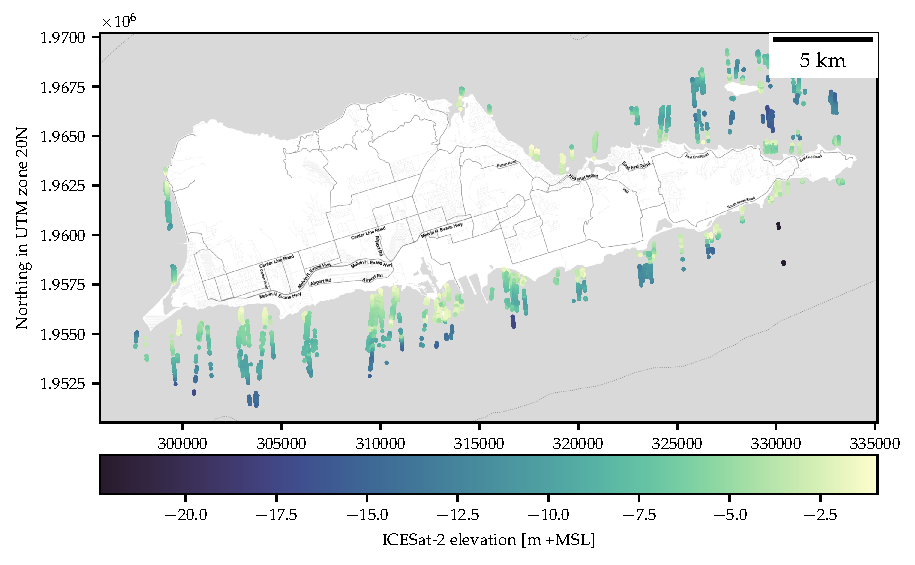
\includegraphics{figures/stcroix_photon_map.pdf}
    \caption{St. Croix site: Identified photons and their depth}
    \label{fig:st-croix-photons}
\end{figure}

The bathymetric point measurements obtained from the KDE signal finding algorithm are shown in \ref{fig:st-croix-photons}. This site showed excellent agreement between the ICESat-2 data and the validation data, and the KDE signal finding algorithm reliably identified bathymetric points as deep as -20m +MSL. The overall RMSE at the site was the lowest of any sites tested, at 0.54m. Figure \ref{fig:st-croix-bias-plot} shows the spread of the ICESat-2 points vs the corresponding point in the validation data.

\begin{figure}[htbp]
    \centering
    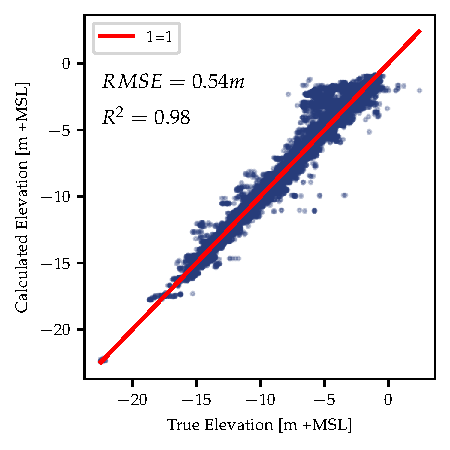
\includegraphics{figures/stcroix_lidar_estimated_vs_truth.pdf}
    \caption{St. Croix site: Identified photons and their depth}
    \label{fig:st-croix-bias-plot}
\end{figure}

After implementing the Kriging/Kalman updating process for the St. Croix site we find that the combination of the kriged ICESat-2 raster with the GEBCO data produces a resulting product that has a higher accuracy than either of the input datasets. Particularly of note here is the inaccuracy of the GEBCO data at this site --- while the overall RMSE of the resulting raster is high at this site compared to some others, in this case it is limited by the accuracy of the starting GEBCO data, and the accuracy of the kriging raster. Table \ref{tab:stcroix_gebco_raster_error} shows the improvement achieved through the Kalman Update process.

\begin{table}
\centering
\caption{Improvement in error metrics after applying Kalman Updating of kriged data}
\label{tab:stcroix_gebco_raster_error}
\begin{tabular}{lrrr}
\toprule
 & RMSE [m] & MAE [m] & Mean Error [m] \\
\midrule
Naive Bilinear Interpolation & 6.45 & 4.30 & -1.01 \\
Kriged Raster & 6.79 & 4.10 & -2.91 \\
Kalman Updated Raster & 4.63 & 3.20 & -1.14 \\
\bottomrule
\end{tabular}
\end{table}


\section{Charlotte Amalie Test site}

\section{Oahu Test sites}

For another validation site that is outside of the Caribbean sea, the island of Oahu in the US state of Hawai'i was chosen. The validation data used is a lidar survey from 2013
\pdfcomment{add more details and citation}. Because this site is substantially larger ($\approx 4x$ the area) than the other test sites, to analyze the data, the coast of the island is first divided into 8 smaller subsites. The layout of these sites was chosen based on approximately similar coastline characteristics. Figure \ref{fig:oahu-subsite-layout} shows the selected distribution of the smaller subsites around the island of Oahu.

\begin{figure}[htbp]
    \centering
    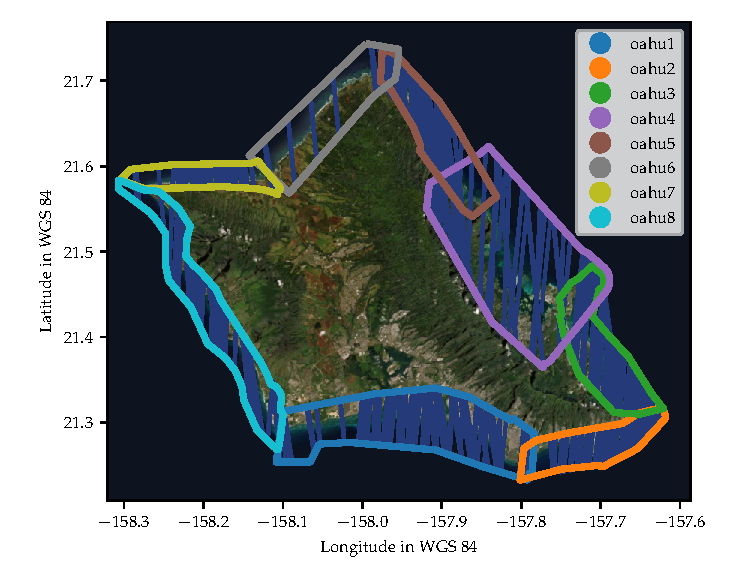
\includegraphics{figures/Oahu_all_tracklines.pdf}
    \caption{Oahu test site: The distribution of the subsites around the island of Oahu. Base layer data provided by: Esri, i-cubed, USDA, USGS, AEX, GeoEye, Getmapping, Aerogrid, IGN, IGP, UPR-EGP, and the GIS User Community}
    \label{fig:oahu-subsite-layout}
\end{figure}

The different subsites also exhibit different hydraulic characteristics. The Northern edge of the island is exposed to longer swells and larger wave heights, while the south is relatively sheltered \parencite{Vitousek2008a}. Another aspect is that distribution of ICESat-2 tracks is not even across all sites. Sites 4 and 6, for example do not contain any ascending \pdfcomment{check ascending/descending} transects with good data, so distribution of the data will be more uneven and might reduce the quality of the kriging raster.

The accuracy of the KDE algorithm derived lidar data points, grouped by subsite, are shown in Table \ref{tab:Oahusitestats}. It can be seen that site 2 has an anomalously high RMS error. 


\begin{figure}
    \begin{floatrow}
    \ffigbox{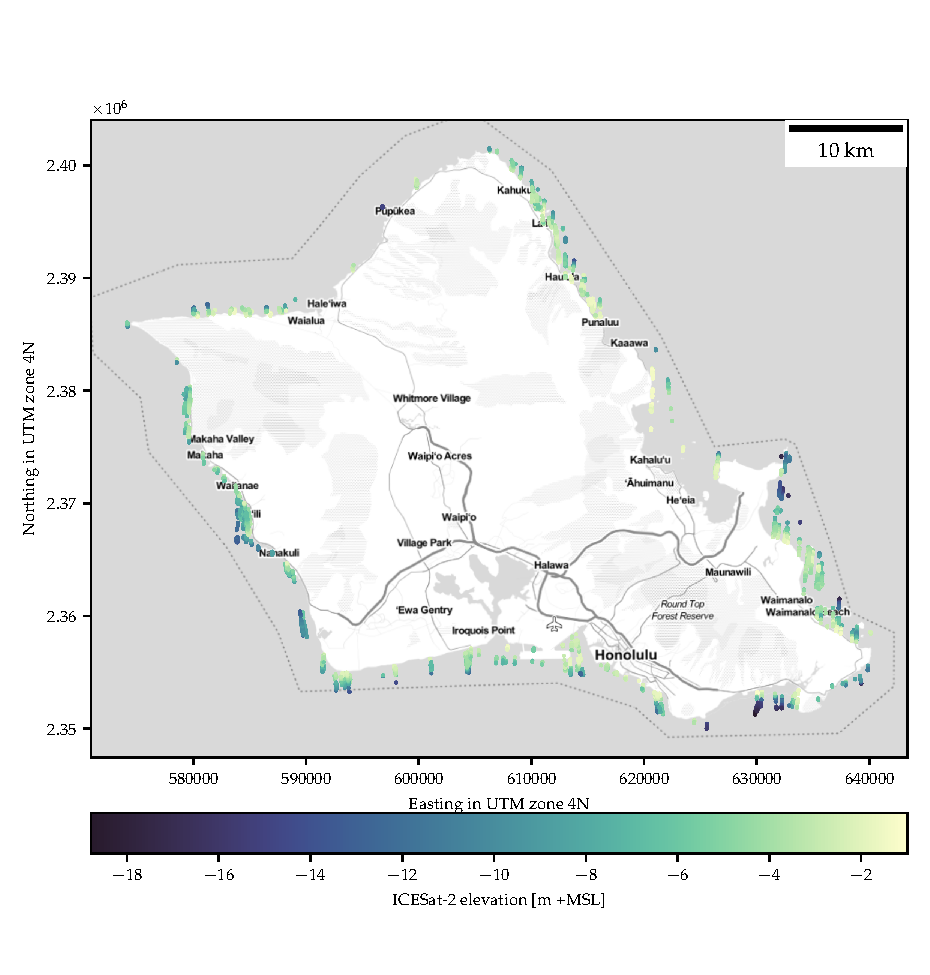
\includegraphics{figures/Oahu_all_sites_photon_points.pdf}}{\caption{Bathymetry point estimates around Oahu from KDE signal finding algorithm}}
    \capbtabbox{%
    \begin{table}[h!]
\caption{Error metrics between ICESat-2 and ground-truth data for all sites in Oahu}
\label{tab:Oahusitestats}
\begin{tabular}{lrrr}
\toprule
 & RMSE & MAE & Count bathy Points Identified \\
Oahu site number &  &  &  \\
\midrule
1 & 1.162525 & 0.768264 & 12775 \\
2 & 10.598899 & 1.447226 & 4327 \\
3 & 1.235144 & 0.463879 & 18566 \\
4 & 0.751631 & 0.565673 & 2738 \\
5 & 0.734813 & 0.504969 & 10443 \\
6 & 2.422447 & 1.756412 & 754 \\
7 & 1.111055 & 0.717672 & 2949 \\
8 & 0.670030 & 0.520755 & 17946 \\
\bottomrule
\end{tabular}
\end{table}

    }{\caption{Error metrics between ICESat-2 and ground-truth data for all sites in Oahu}
    }
    \end{floatrow}
\end{figure}


The cause of this is a weakness in the subsurface filtering process \pdfcomment{add figure}. In there case, there is a small mountain protruding from the sea that is not captured by the low-resolution of the GEBCO grid. As this area of the transect occurs on land, it should be filtered out. However, because it is not filtered out there are several points where noise points under the mountains are included, and they are not filtered out by the KDE threshold, so they are inadvertently included. 

Figures \ref{fig:oahu-bias-mountains} and \ref{fig:oahu-bias-nomounts} show all ICESat-2 bathymetric points in all Oahu Subsites. Figure \ref{fig:oahu-bias-nomounts} has had the scale adjust so that these extreme errors are not visible. This better shows the distribution of the other errors \pdfcomment{rephrase lmao}.

The Kalman update step was also applied individually to each subsite. The Kalman updating step for the various Oahu subsites shows a more mixed result than in other test sites. A summary of the changes in the error metrics for each subsite is provided in Table \ref{tab:oahu-percent-change}. In some sites, the Kalman update does not improve the estimate, and in some cases even makes it than the a-priori GEBCO estimate. This is an indication that the parameters are not set correctly for the site --- using bayesian estimation, the parameters should be able to be set such that areas within the grid that have lower confidence are not changed significantly. 

By manually investigating the results of subsites 6, 7 and 8 there is some indication of what is going wrong to produce these results. The 

% \begin{table}[htbp]
% \centering
% \caption{Percent reduction in error metrics via the Kalman updating approach. Positive values indicate reduced error, negative ones indicate increased error.}
% \label{tab:oahu-percent-change}
\begin{tabular}{lrrr}
\toprule
Subsite &  RMSE Change & MAE Change & Mean Error Change \\
\midrule
1 & 38.43\% & 38.75\% & 53.46\% \\
2 & 31.62\% & 29.61\% & 51.10\% \\
3 & 25.18\% & 22.68\% & 75.06\% \\
4 & -1.76\% & -1.01\% & 123.78\% \\
5 & 1.94\% & 4.52\% & 116.88\% \\
6 & -18.14\% & -16.12\% & -14.68\% \\
7 & -22.61\% & -15.04\% & -16.58\% \\
8 & -25.15\% & -21.05\% & -544.94\% \\
\bottomrule
\end{tabular}
% \end{table}


\begin{figure}
    \begin{floatrow}
        \ffigbox{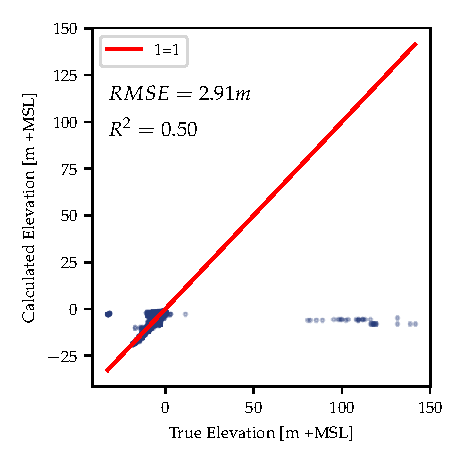
\includegraphics{figures/Oahu_combined_lidar_estimated_vs_truth.pdf}}{\caption{Bias plot of all points within all Oahu Subsites}\label{fig:oahu-bias-mountains}}
        \ffigbox{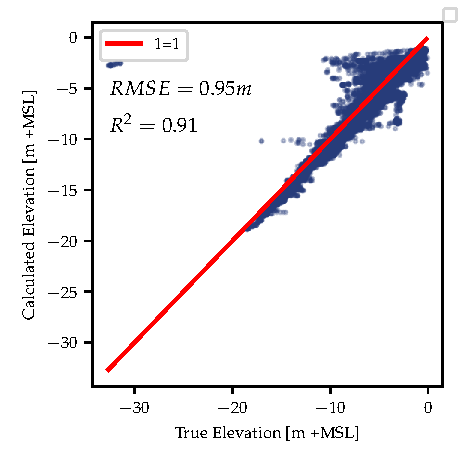
\includegraphics{figures/Oahu_combined_mountains_removed_lidar_estimated_vs_truth.pdf}}{\caption{Bias plot with the mountain points removed to better show the actual distribution of the error}\label{fig:oahu-bias-nomounts}}
    \end{floatrow}
\end{figure}



\section{All sites combined}

\subsection{Lidar error}

\subsection{Kalman updating approach }

% \subsection{Site Conditions Summary}
% \begin{table}[h!]
%     \begin{minipage}{0.5\textwidth}
%         \centering\begin{tabular}{r l }
%             Parameter                                                 & \textbf{Value}                  \\
%             \hline
%             Location                                                  &                                 \\
%             Tidal Range \footcite{Tidal_data_reanalysis2022}          & \qty{2.24}{m}                   \\
%             Average Secchi Depth \footcite{ACRI-STGlobColourTeam2020} & \qty{3.86}{m}                   \\
%             Validation Data vertical RMS error                        & \qty{}{m} \pdfcomment{look up}  \\
%             Validation Data Horizontal Resolution                     & \qty{}{m} \pdfcomment{look up?} \\
%             Vertical Datum                                            & Normaal Amsterdams Peil (NAP)   \\
%         \end{tabular}
%     \end{minipage}
%     \caption{Site conditions for the Florida Keys site}
%     \label{table:Pettensitestats}
% \end{table}

% \subsection{Validation data}
% The validation data for this site was from a 2021 survey performed by Van Oord.
% \subsection{Error Jarkus Vs. Survey}
% There was some error between the Jarkus survey points and the Van Oord 1m surveyed grid. The error metrics are shown in table \ref{tab:jarkus_vs_survey_error}, and the distribution of the error is shown in figure
% \begin{table}[h!]
\caption{Error between Surveyed Bathymetry grid and Jarkus}
\label{tab:jarkus_vs_survey_error}
\begin{tabular}{lrr}
\toprule
 & MAE & RMSE \\
\midrule
Petten & 0.267152 & 0.439663 \\
\bottomrule
\end{tabular}
\end{table}


% \begin{figure}[h]
%     \centering
%     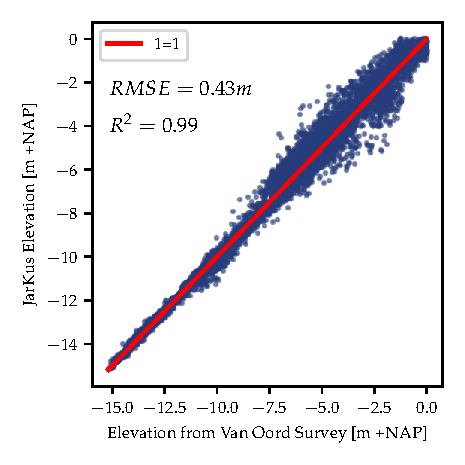
\includegraphics{figures/petten_lidar_estimated_vs_truth.pdf}
%     \caption{Jarkus Survey points vs same location on Van Oord Survey data}
%     \label{fig:jarkus_vs_survey}
% \end{figure}

% \subsection{Jarkus data kriging and Kalman update}
% \begin{table}[h!]
\caption{Improvement in Error when incorporating Kriged Jarkus data}
\label{tab:jarkus_kriging_kalman_error}
\begin{tabular}{lrr}
\toprule
 & RMSE & MAE \\
\midrule
Naive Bilinear Interpolation & 1.473726 & 1.311282 \\
Kalman Updated Raster & 0.722669 & 0.483035 \\
Kriged Raster & 0.743263 & 0.496904 \\
\bottomrule
\end{tabular}
\end{table}


% \section{Marathon Key Test Site}

% \begin{table}[h]
%     \begin{minipage}{0.5\textwidth}
%         \centering\begin{tabular}{r l }
%             Parameter                                                      & \textbf{Value}                                 \\
%             \hline
%             Location                                                       & -81.04472,24.72868                             \\
%             Tidal Range \footcite{Tidal_data_reanalysis2022}               & \qty{0.51}{m}                                  \\
%             Average Secchi Depth \footcite{ACRI-STGlobColourTeam2020}      & \qty{0.0}{m}                                   \\
%             Validation Data Vertical RMS error \footcite{Keys2019Lidar}    & \qty{0.056}{m}                                 \\
%             Validation Data Horizontal Resolution \footcite{Keys2019Lidar} & \qty{9.4e-6}{ \degree} $\approx$ \qty{0.95}{m} \\
%             Vertical Datum \footcite{Keys2019Lidar}                        & local MSL                                      \\
%         \end{tabular}
%     \end{minipage}
%     \caption{Site conditions for the Florida Keys site}
%     \label{table:floridasitestats}
% \end{table}


% \subsection{ICESat-2 Transects within AOI}
% The AOI used the validate the method is shown in figure \ref{fig:keys_transects} below.
% \begin{figure}[h]
%     \centering
%     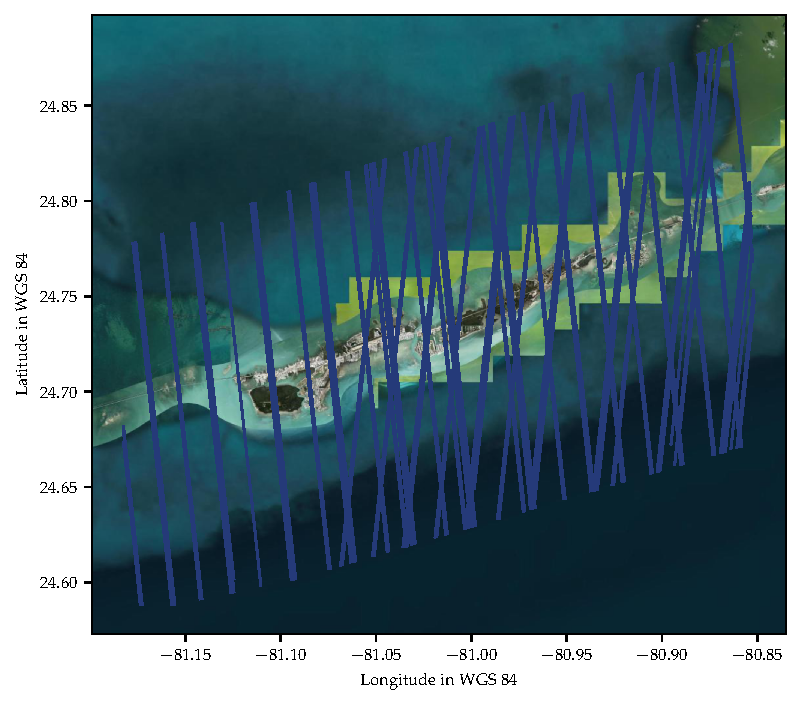
\includegraphics{figures/florida_keys_tracklines.pdf}
%     % \input{figures/study_site_tracklines.pgf}
%     \caption{Location of ICESat-2 Transects in Florida keys Study Area}
%     \label{fig:keys_transects}
% \end{figure}
% \subsection{Validation Data}
% The validation data used for this site is from a detailed lidar survey of the area performed in 2018 and 2019 by Quantum Spatial, Inc. \parencite{Keys2019Lidar}. The survey was performed using a Riegl VQ-880-G hydrographic airborne laser scanner. The instrument is designed for high bathymetric accuracy in shallow water.

% \subsection{Bathymetric Signal finding}
% Figure \ref{fig:keys-photons} shows the location and estimated bathymetric depths of individual ICESat-2 photon returns.
% \begin{figure}[h]
%     \centering
%     \includegraphics{figures/Florida_keys_photon_map.pdf}
%     \caption{Geographic distribution of Bathymetric photon data}
%     \label{fig:keys-photons}
% \end{figure}

% \subsection{Lidar updated GEBCO vs. Simple bilinear Interpolation}
% The results when comparing a raw interpolation of GEBCO to
% \begin{table}
\centering
\caption{Improvement in error metrics after applying Kalman Updating of kriged data}
\label{tab:florida_keys_gebco_raster_error}
\begin{tabular}{lrr}
\toprule
 & RMSE & MAE \\
\midrule
Naive Bilinear Interpolation & 2.21 & 1.11 \\
Kalman Updated Raster & 1.41 & 0.85 \\
Kriged Raster & 2.28 & 1.31 \\
\bottomrule
\end{tabular}
\end{table}



% \section{St. Croix}

% \subsection{Site Characteristics}

% St. Croix is in the US Virgin Islands. \pdfcomment{flesh out}

% \begin{figure}[h]
%     \centering
%     \includegraphics[width=\textwidth]{figures/Stcroix_tracklines.pdf}
%     \caption{ICESat-2 tracklines available in the St. Croix site}
%     \label{fig:st-croix-tracklines}
% \end{figure}

% \subsection{ICESat-2 Signal Extraction}
% After downloading the above tracklines and processing them, the points shown in were identified by the algorithm as containing bathymetric measurements.

% \begin{figure}[h]
%     \centering
%     \includegraphics[width=\textwidth]{figures/Stcroix_photon_map.pdf}
%     \caption{Point estimates of bathymetry from KDE algorithm}
%     \label{fig:stcroix-bathy-points}
% \end{figure}

% This site showed excellent agreement between the point ICESat-2 estimated lidar and the validation data. The error metrics are shown in table \ref{tab:stcroix_lidar_error}

% \begin{table}[h!]
\caption{Error between the point bathymetry and ground-truth data}
\label{tab:stcroix_lidar_error}
\begin{tabular}{lrrrrr}
\toprule
 & MAE & RMSE & Median Abs error & R2 Score & Average Error \\
\midrule
stcroix & 0.299882 & 0.545965 & 0.176959 & 0.975837 & -0.087435 \\
\bottomrule
\end{tabular}
\end{table}


% \subsection{GEBCO Updating}

% The change in the error metrics that is provided by the  is shown in table \ref{tab:stcroix-raster-error}

% \begin{table}
\centering
\caption{Improvement in error metrics after applying Kalman Updating of kriged data}
\label{tab:stcroix_gebco_raster_error}
\begin{tabular}{lrrr}
\toprule
 & RMSE [m] & MAE [m] & Mean Error [m] \\
\midrule
Naive Bilinear Interpolation & 6.45 & 4.30 & -1.01 \\
Kriged Raster & 6.79 & 4.10 & -2.91 \\
Kalman Updated Raster & 4.63 & 3.20 & -1.14 \\
\bottomrule
\end{tabular}
\end{table}


% \section{Charlotte Amalie}
% Another test site is the island of Charlotte Amalie in the US Virgin Islands. Basic details about the test site are in \ref{table:charlotteamalie_datatable}
% \begin{table}[h]
%     \begin{minipage}{0.5\textwidth}\pdfcomment{fill in table}
%         \centering\begin{tabular}{r l }
%             Parameter                                                 & \textbf{Value} \\
%             \hline
%             Location                                                  &                \\
%             Tidal Range \footcite{Tidal_data_reanalysis2022}          & \qty{}{m}      \\
%             Average Secchi Depth \footcite{ACRI-STGlobColourTeam2020} & \qty{}{m}      \\
%             Validation Data vertical 95\% confidence                  & $x$ m          \\
%             Validation Data Horizontal Resolution                     & \qty{}{m}      \\
%             Vertical Datum                                            & lookup         \\
%         \end{tabular}
%     \end{minipage}
%     \caption{Site conditions for the Charlotte Amalie}
%     \label{table:charlotteamalie_datatable}
% \end{table}
% Overall there where X \pdfcomment{lookup number of transects} transects of ICESat-2 data available for the site, and their distribution is shown in figure \ref{fig:charlotteamalietracklines}.

% \begin{figure}[h]
%     \centering
%     \includegraphics[width=\textwidth]{figures/Charlotteamalie_tracklines.pdf}
%     \caption{ICESat-2 tracks in the Charlotte Amalie Test site}
%     \label{fig:charlotteamalietracklines}
% \end{figure}

% \subsection{Lidar Points found for site}
% Figure \ref{fig:pointmapcharlotteamalie} shows the geographic distribution of the points

% \begin{figure}[h]
%     \centering
%     \includegraphics[width=\textwidth]{figures/Charlotteamalie_photon_map.pdf}
%     \caption{Charlotte Amalie points}
%     \label{fig:pointmapcharlotteamalie}
% \end{figure}

% The error for the site is shown in \ref{fig:charlotteamalie-lidar-bias}

% \begin{figure}[h]
%     \centering
%     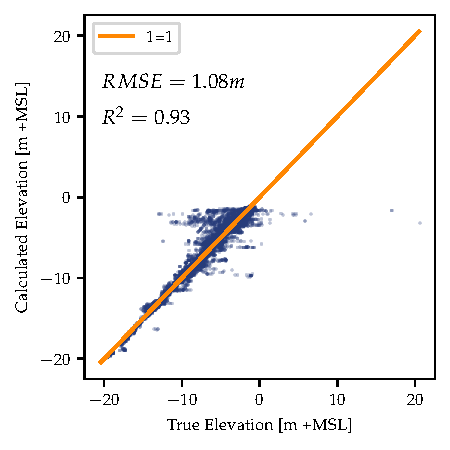
\includegraphics{figures/charlotteamalie_lidar_estimated_vs_truth.pdf}
%     \caption{Bias plot showing the agreement between the validation data and the lidar points for Charlotte Amalie}
%     \label{fig:charlotteamalie-lidar-bias}
% \end{figure}


% \section{Oahu}
% One test site that was selected based on the clear water and the high quality validation data is the Island of Oahu, in the US state of Hawai'i. The island has an extremely varied shelf and coastal environment along its length, to it provides the ability to test the results in in areas with a variety of offshore slopes and wave energy environments.

% Because of the size of the island, the nearshore zone was divided into 8 different zones, for which the data was downloaded and processed seperately. The results were then combined and summarized. A map of the area that shows the available ICESat-2 tracklines and the subareas used to download the and process the data are shown in figure \ref{fig:oahu-all-sites-transects}

% \begin{figure}[h]
%     \centering
%     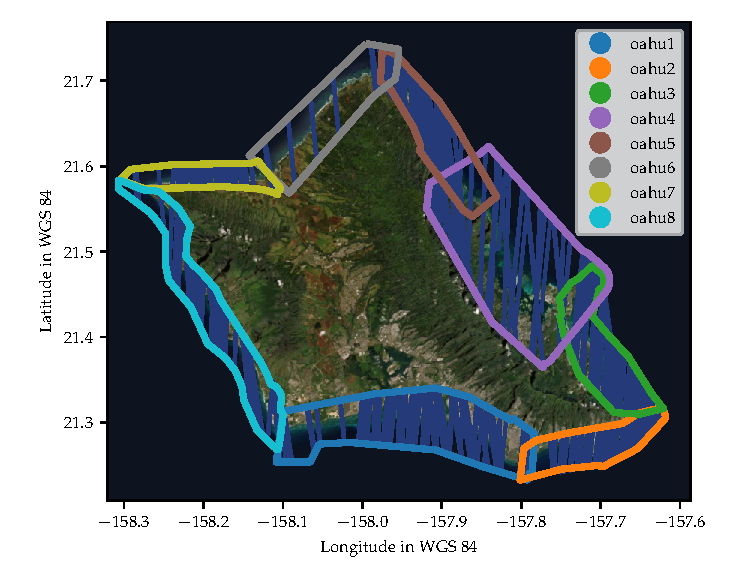
\includegraphics[width=\textwidth]{figures/Oahu_all_tracklines.pdf}
%     \caption{Transects and subsite distribution for Oahu Test site}
%     \label{fig:oahu-all-sites-transects}
% \end{figure}

% \subsection{ICESat-2 Signal Extraction}

% The data for all 8 subsites was downloaded and the filtering and KDE signal finding steps were applied. Figure \ref{fig:oahu-all-photon-map} shows the spatial distribution

% \begin{figure}[h]
%     \centering
%     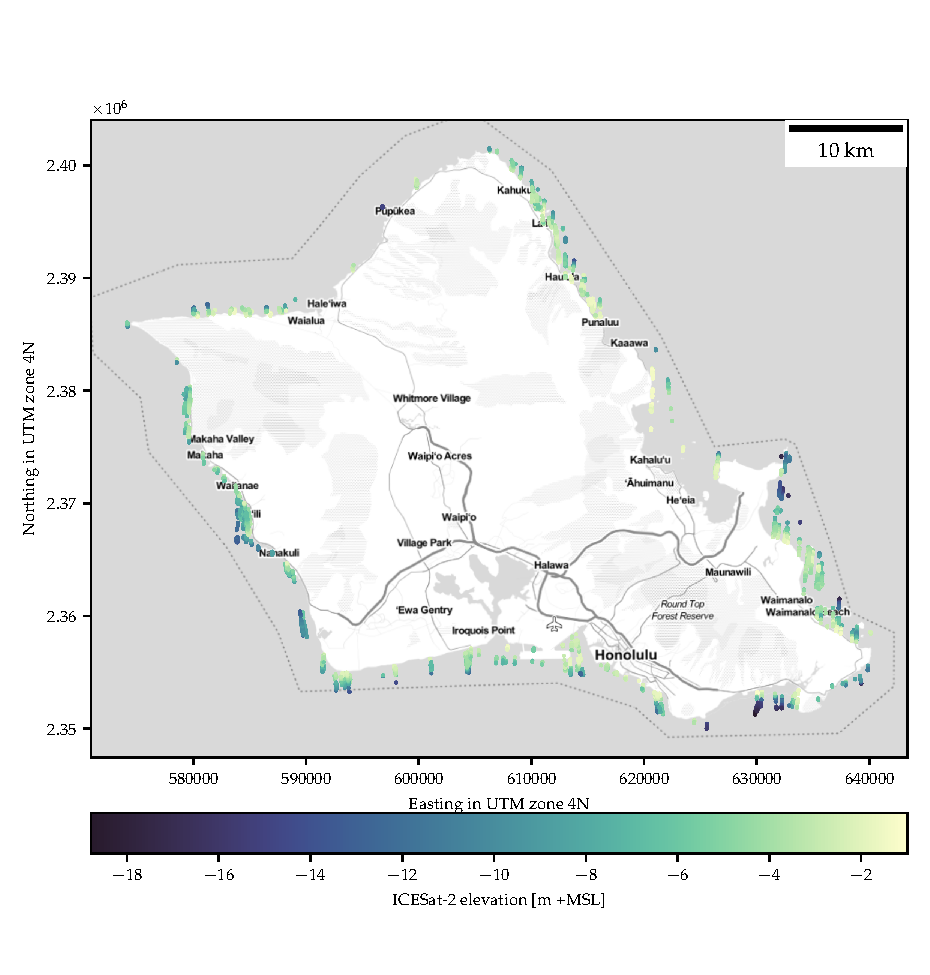
\includegraphics[width=\textwidth]{figures/Oahu_all_sites_photon_points.pdf}
%     \caption{The layout of the identified bathymetry point measurements around Oahu}
%     \label{fig:oahu-all-photon-map}
% \end{figure}

% The sites varied significantly in in the accuracy of the ICESat-2 point bathymetry. Some sites showed a significant RMS error due to the presence of mountain peaks up to a few hundred meters high with small horizontal footprint. These features are not captured by the GEBCO grid and therefore photon returns below them are not filtered due to the GEBCO-based horizontal filtering. Table \ref{table:Oahusitestats} contains the compiled error metrics for each site.

% \pdfcomment{add to discussion section} \pdfcomment{good to explain with a figure I think}

% \begin{table}[h!]
\caption{Error metrics between ICESat-2 and ground-truth data for all sites in Oahu}
\label{tab:Oahusitestats}
\begin{tabular}{lrrr}
\toprule
 & RMSE & MAE & Count bathy Points Identified \\
Oahu site number &  &  &  \\
\midrule
1 & 1.162525 & 0.768264 & 12775 \\
2 & 10.598899 & 1.447226 & 4327 \\
3 & 1.235144 & 0.463879 & 18566 \\
4 & 0.751631 & 0.565673 & 2738 \\
5 & 0.734813 & 0.504969 & 10443 \\
6 & 2.422447 & 1.756412 & 754 \\
7 & 1.111055 & 0.717672 & 2949 \\
8 & 0.670030 & 0.520755 & 17946 \\
\bottomrule
\end{tabular}
\end{table}


% The overall bias plot showing all the subsites is shown in figure \ref{fig:oahu-all-bias-plot}

% \begin{figure}[h]
%     \centering
%     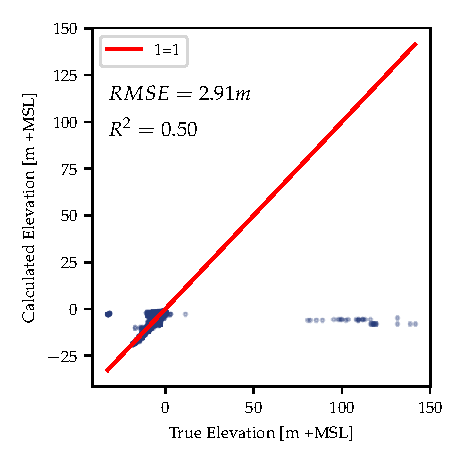
\includegraphics[width=0.7\textwidth]{figures/Oahu_combined_lidar_estimated_vs_truth.pdf}
%     \caption{Bias plot for all Oahu subsites combined}
%     \label{fig:oahu-all-bias-plot}
% \end{figure}

% The reason the RMSE at site 2 is much higher than the rest is that there was a mountain of 120m tall that was in the validation data. If that is removed, the error drops significantly. 


% \pdfcomment{these two figures could be combined into subplots probably }
% \begin{figure}[h]
%     \centering
%     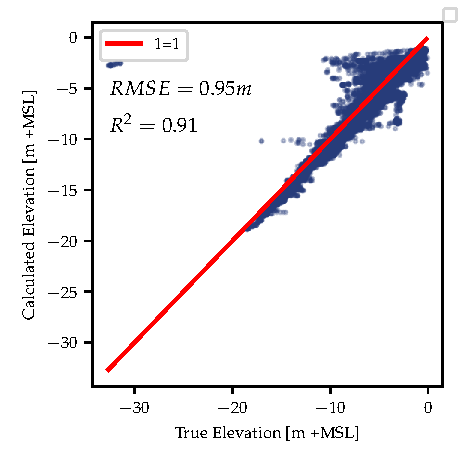
\includegraphics[width=0.7\textwidth]{figures/Oahu_combined_mountains_removed_lidar_estimated_vs_truth.pdf}
%     \caption{Oahu - all sites with mountain removed}
%     \label{fig:oahu-bias-no-mountains}
% \end{figure}

% To better show the distribution of the error smaller errors, figure \ref{fig:oahu-bias-no-mountains} shows the same combination of points, but with the outlier values 

% \subsection{Kalman Updating}

% \section{Summary}
% The results of all the test sites that used lidar data were combined into a single bias plot shown in figure \ref{fig:all-sites-biasplot}

% \subsection{ICESat-2 error}

% \begin{figure}[h]
%     \centering
%     \includegraphics[width=0.7\textwidth]{figures/all_site_combined_biasplot.pdf}
%     \caption{All lidar points for all sites with validation data}
%     \label{fig:all-sites-biasplot}
% \end{figure}

% \section{Water clarity metrics}


% \begin{figure}[ht]
%     \centering
%     \includegraphics{figures/secchi_by_site_boxplot.pdf}
%     \caption{The distribution of Secchi depth along transects during the time of ICESat-2 transects}\pdfcomment{fix xtick labels and make site names fancier}
%     \label{fig:secchi-boxplot}
% \end{figure}
